\documentclass[11pt,letter]{article}
\usepackage[top=0.30in, bottom=0.7in, left=1.1in, right=1.1in]{geometry}
\usepackage{graphicx} % Required for inserting images
\usepackage{xcolor} 
\usepackage{amsmath}
\usepackage{gensymb}
\definecolor{Accent}{HTML}{bd2b00} 
\usepackage{natbib}
\usepackage{hyperref}
\hypersetup{colorlinks,citecolor = Accent, linkcolor = Accent,urlcolor = Accent, breaklinks=true}
\usepackage{cleveref}
\usepackage[labelfont=bf]{caption}
\bibliographystyle{amnat}

\RequirePackage[labelfont={bf,sf},%
                font={small, sf}]{caption}


\let\oldthefigure\thefigure
\renewcommand{\thefigure}{S\oldthefigure}

\begin{document}

\title{Solstice optimizes thermal growing season\\\emph{Supplementary figures}}
\author{Victor Van der Meersch$^{1}$, E. M. Wolkovich$^{1}$}
\date{}
\maketitle 

\begin{figure}[h]
	\hspace*{-1.4cm}
	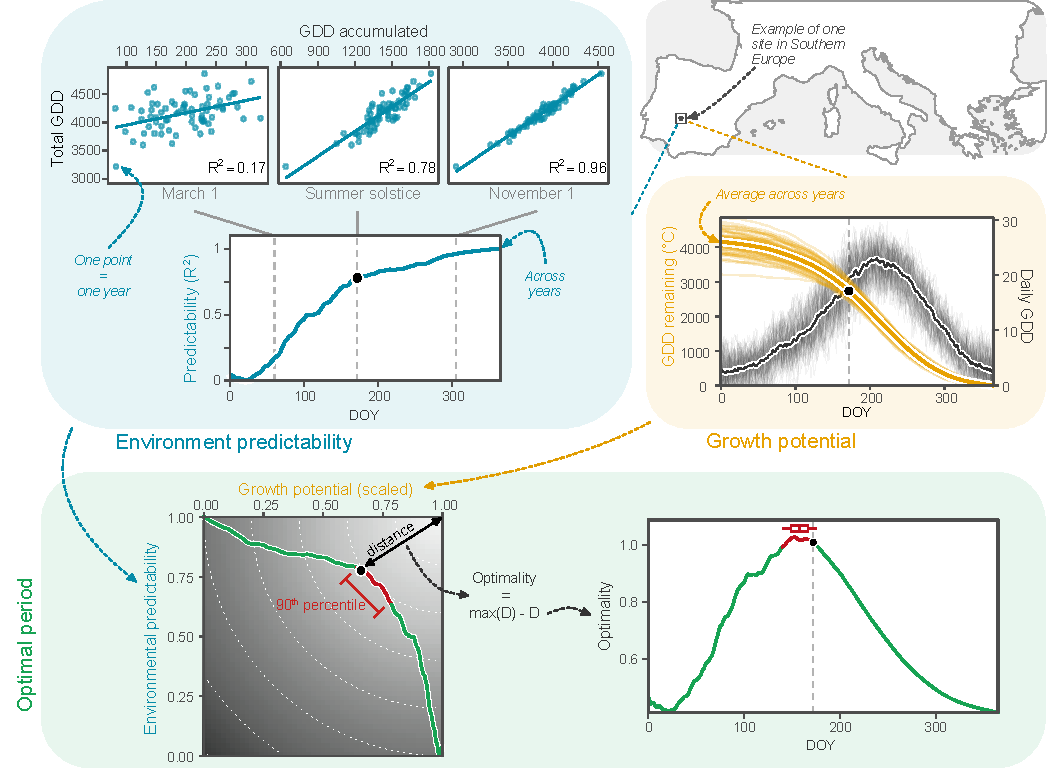
\includegraphics{../suppmat/method_figure.pdf}
	\vspace*{-0.4cm}
	\caption{\textbf{Workflow of the optimality analysis for one site in Southern Europe.}} 
	\label{fig:method}
\end{figure}
\clearpage

\begin{figure}
	\centering
	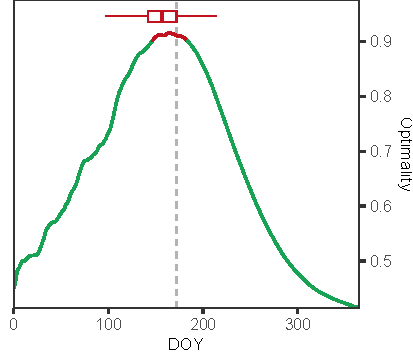
\includegraphics[scale = .9]{../suppmat/global_optimality_0_40.pdf}
	\vspace*{-0.cm}
	\caption{\textbf{Average optimal trade-off between environmental predictability and growth potential across Europe, with an alternative GDD definition} ($T_{lower}=0$\degree C and $T_{upper}=40$\degree C).}
	\label{fig:altgdd}
\end{figure}

\begin{figure}
	\centering
	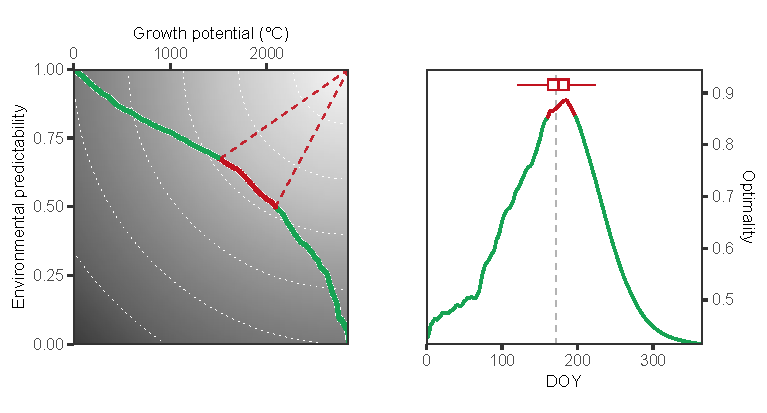
\includegraphics[scale = 1]{../suppmat/global_optimality_northamerica.pdf}
	\vspace*{-0.2cm}
	\caption{\textbf{Solstice also marks the average optimal trade-off between environmental predictability and growth potential across North America (1951-2020).} The red sections of the green curves represent days where optimality falls within the 90th percentile (i.e. top 10\% most optimal days).}
	\label{fig:global_norame}
\end{figure}

\begin{figure}
	\centering
	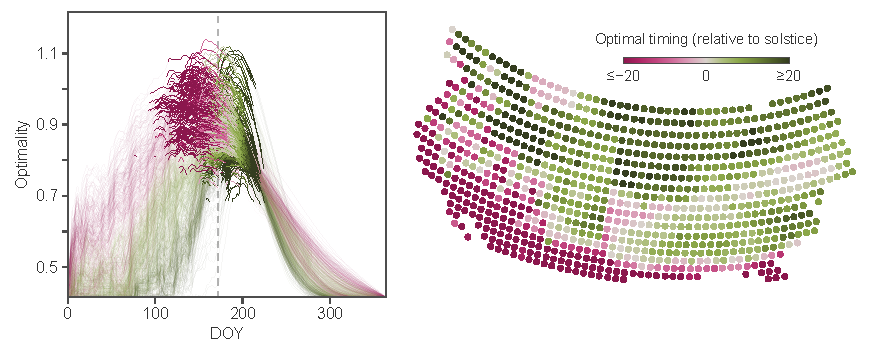
\includegraphics[scale = 1]{../suppmat/local_optimality_norame.pdf}
	\vspace*{-0.2cm}
	\caption{\textbf{Average optimal timing (\Cref{fig:global_norame}) hides variation in optimal timing across the different climatic conditions of North America (1951-2020).} On the left panel, each curve shows the optimality for a given site. Sites are sampled on a regular grid across Europe, as shown on the central map. Colors indicate the timing---relative to the solstice---of the median optimal day.}
	\label{fig:local_norame}
\end{figure}

\begin{figure}
	\centering
	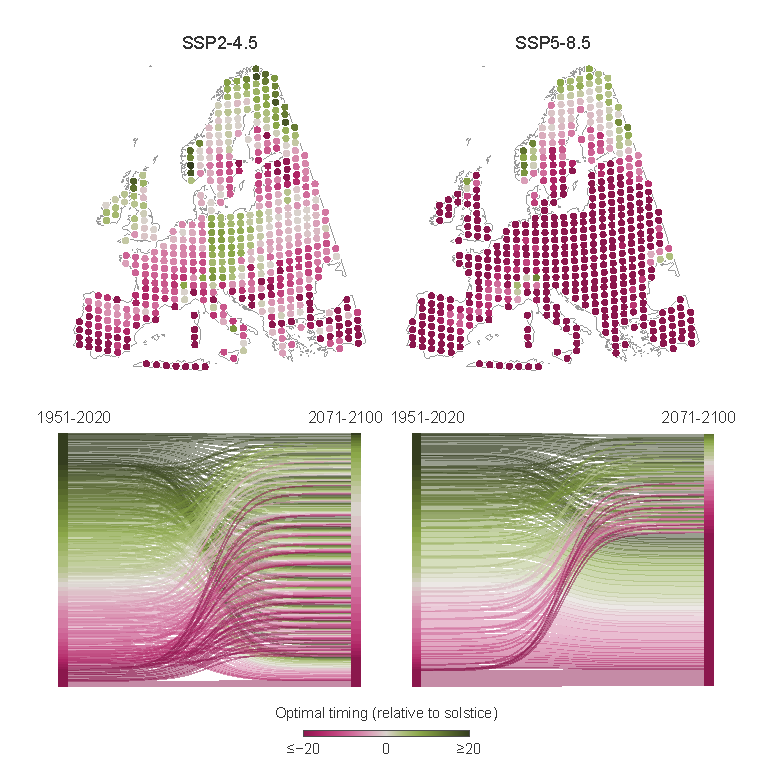
\includegraphics[scale = 1]{../suppmat/local_optimality_future.pdf}
	\vspace*{0.3cm}
	\caption{\textbf{Average optimal timing (\Cref{fig:globaloptimality}) hides variation in optimal timing across the different future climatic conditions of Europe (2071-2100).} On the top panel, sites are sampled on a regular grid across Europe. On the bottom panel, Sankey diagrams show the proportional flow of (site-specific) optimal timing from 1951-2020 to 2071-2100. Colors indicate the timing—relative to the solstice—of the median optimal day.}
	\label{fig:futurelocal}
\end{figure}


\end{document}

